\chapter{Background} \label{ch:background}

This chapter provides an extensive discussion on network control in packet
switched networks.  We motivate the discussion on network control, describing
the architecture of network devices and their inherent physical
limitations~(Section~\ref{sec:background:forwarding}) and elaborate on existing
network control mechanisms for production networks, focusing on some of their
deficiencies~(Section~\ref{sec:background:netcontrol}).  Furthermore, we present
three important network control frameworks, namely Active Networks, Devolved
Control of ATM Networks~(DCAN) and Software Defined Networking (SDN), proposed
by the research community to address some of the limitation
of current control schemes~(Section~\ref{sec:background:netcontrol}). Finally,
we focus on the most recent control framework, SDN, and present some of its
applications in modern network problems~(Section~\ref{sec:background:ofapp}).

\section{Forwarding Devices} \label{sec:background:forwarding}

Packet networks have become a \emph{'de-facto'} approach in communication
networks. Their success relies, to a great extend, on the offered high medium
utilization and low-cost design principle.  Packet-switched networks can
function over a large set of physical layer technologies and replace tradition
connection-oriented mechanisms (e.g.~telephony, TV broadcast). In this section
we focus on Ethernet and IP networks, the predominant protocol implementations
for packet networks, and provide a design overview of a hardware \emph{Switch},
a typical forwarding device.  
% Providing a high level
% insight on the architecture of a Switch, can highlight the existing lower bounds
% on the functionality and extendibility of such devices. 

\begin{figure}
  \centering
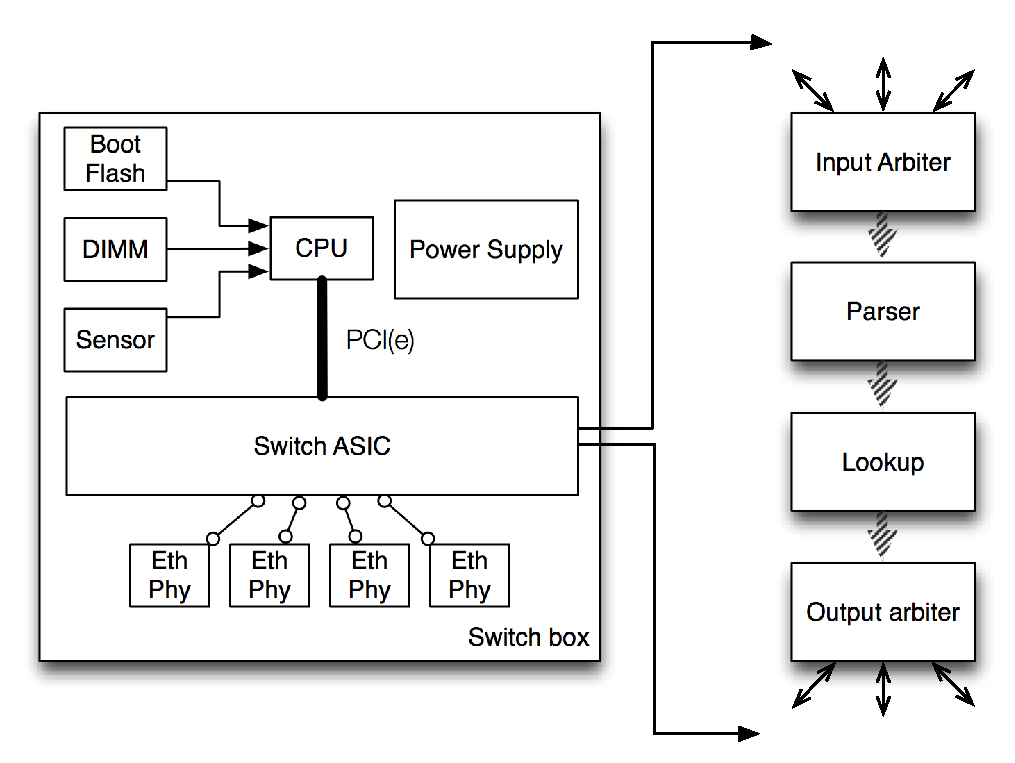
\includegraphics[width=0.6\textwidth]{Background/BackgroundFigs/switch_design}
\caption{A generic architecture of a Switching device.}
\label{fig:background:switch_design}
\end{figure}

Network switches are the main mechanism to multiplex Ethernet links.  Their main
functionality provides collision-free connectivity between network segments.
Nonetheless, as the network complexity increases, switches augment their
functional roles in a network and their hardware architecture is highly diverse. For
example, unmanaged switches provide a low cost non-configurable interconnection
device for small networks, supporting usually a few 1 gig ports, while
distribution switches are used in large enterprise networks to interconnect
aggregation switches, support multiple 10 or 40 Gig links and provide multiple
mechanisms to inspect and control network traffic.  In this section we will use
the Top-of-Rach~(ToR) switch type as an reference to elaborate on the
architecture of modern switches. 
Such switches are used in datacenter networks to aggregate traffic between the
edge and the distribution network layers.  TOR switches commonly use a single
Application-Specific Integrated Circuits~(ASIC) silicon and can forward
high-rate traffic non-blocking at line rate.  As presented in
Figure~\ref{fig:background:switch_design}, a typical switch device consists of
the following components:

\begin{itemize}
  \item \emph{management CPU}: Switch boxes contain a programmable CPU, which
        runs the control plane logic and provide configurability. Switch CPUs
        usually run a simple operating system and communicate with the switch
        ASICs in order to modify their functionality, based on the policy.
        Switch vendors usually use low-power CPUs, such as SoC PowerPC chips or
        even ARM and MIPS CPUs. The CPU can access runtime memory modules (Boot
        Flash and RAM), to store transient state, and persistent memory (e.g.~SD
        Cards) through memory extension slots, to store log files and
        configuration. In general, switch CPUs provide sufficient computation
        resources to run the switch control-plane functionality, but they cannot
        accommodate intensive processing tasks. The OS provide network services,
        like telnet and SSH, to provide a command line interface to network
        managers, while usually it also provides SNMP services to aggregate
        switch statistics. 
 
  \item \emph{Switch ASIC}: The switch ASIC~\cite{hp-asic,broadcom-asic,intel-asic}
        implements in hardware the forwarding plane of the switch.  The
        capabilities of an ASIC are variable, depending on the vendor and the
        cost, but define the performance limits of the device to handle data
        plane traffic.
        Implementation details of an ASIC silicon remain usually concealed, as
        they constitute an important asset for the producer.  The design of
        an ASIC is an expensive process, as their design and testing period is
        long and requires significant human labour and material
        resources. As a result, switch silicon innovation has a high latency to
        reach the production environment. Furthermore, as in general purpose CPU 
        design,  the processing capacity of an ASIC is upper bound by the
        transistor density and size.

        TOR-type switches can handle line-rate non-blocking traffic for a number
        of ports, using a single ASIC silicon.  An ASIC contains four important
        modules.  The \emph{input arbiter} module multiplexes and synchronizes
        packets from the Ethernet ports to the main processing pipeline of the
        silicon. The arbiter ensures non-preemptive packet processing, by
        bridging the rate mismatch between the silicon processing clock and the
        link rate.  In the main processing pipeline the ASIC contains at least a
        \emph{protocol parsing} module and an \emph{memory lookup} module. The
        protocol parser extracts significant packet fields from network packets
        and the memory lookup module uses the packet fields to define the packet
        processing and forwarding operations.  The lookup module relies on an
        interface with an external memory module in order to match protocol
        fields with forwarding policy.  Memory modules have a trade-off between
        cost and access speed and between memory cost and memory management
        complexity~\footnote{CAM/TCAM lookup: $<$ 10 clock cycles, SRAM: 2-3 nsec,
          DRAM: 20-35
          nsec,~\url{http://people.ee.duke.edu/~sorin/prior-courses/ece152-spring2009/lectures/6.2.2-memory.pdf}}.
        Finally, the \emph{output arbiter} module is responsible to apply
        modifications to the packet and forward it to the appropriate output
        queue. Beyond the aforementioned modules, an ASIC may have additional
        processing modules in the main packet processing pipeline, to extend its
        functionality with operations like access control list (ACL) virtual
        network queues and flow
        statistics monitoring.

  \item \emph{ASIC-CPU communication}: The switch CPU is connected with the ASIC
        over a PCI or PCI-express bus. The communication channel provides an
        elementary bi-directional channel: the CPU controls ASICs registers, to
        modify forwarding functionality, and the ASIC propagates information for
        exceptional states to the CPU. The channel provides sufficient bandwidth
        for basic control plane communication, but it is not designed to handle
        high rate information.

  \item \emph{Memory}: Apart for the in-ASIC memory modules, modern switches
        also use multiple memory types to support the run-time requirements of
        the firmware. A switch is usually equipped with CPU Boot Flash,
        to boot the OS/firmware, DIMM RAM and multiple memory slots,
        for control plane logging and configuration persistence.

  \item \emph{Ethernet ports} : The receipt and transmission of Ethernet packets
        is implemented as a separate hardware circuit. The module is responsible
        to implement the physical layer and MAC layer protocol and propagates
        packets to the ASICs using a  Media Independent Interface (MII).  The
        phy module  usually contains small packet buffers to reduce packet
        losses for bursty traffic.  
\end{itemize}

The physical limitation for the control plane are defined by the ability of the
management CPU to communicate with the ASIC. This communication can be further
characterised by the speed of the switch to read and write ASIC registers and
modify the ASIC memory modules. In addition, the computational requirement of
the control plane logic can impact severely the control plane performance, if
the management CPU processing capacity is limited. 

TOR switches are simple switch devices,  supporting the traffic requirements of
the edge network and provide low to medium forwarding capacity. As we move
closer to the core of the network, the processing capacity requirements, as well
as, device complexity are increased. Multi-chassis switches and routers cannot
contain the required functionality in a single ASIC. Packet processing is
distributed between multiple silicons, complex clos interconnection crossbars
are used to provide non-blocking Terabit backplane
capacity~\cite{juniper_t_series} and the complexity of the control plane to
modify forwarding policy is increased. In addition, providing fast address
lookup requires multiple distributed buffers and cache coherent protocols to
ensure state consistency~\cite{cisco_cef}. For these classes of devices, the
control plane abstraction has a complex and slow translation to ASIC management
operations and programming flexibility is restricted.  

% Higher-end chassis Switches, employ more complex architectures 
% to support Terrabyte traffic rates, using multi-step packet processing and
% connection redundacy. Because their processing and forwarding capabilities can
% match the capabilities of routers, their architecture is similar to high-end
% switch. 
% An extensive discussion over hardware architecture of
% older high-end Cisco switches is presented in~\cite{cisco-routers}.

\section{Forwarding Control in Production Networks} \label{sec:background:netcontrol}

% In this section, we
% present the Data Link and Network layer protocols used in current production
% networks for dynamic control and discuss their limitations
% 
% \subsection{Routing and switching}

Dynamic network control has been an important functionality for computer network
technologies. Forwarding devices require mechanism to automate forwarding logic
update when network state changes in order to ensure end-to-end connectivity.
Existing standardized approaches aim for {\it distributed}, {\it autonomous} and
{\it resilient} network control and are influenced extensively by the end-to-end
principle of the Internet. A switch or a router control functionality requires
only local forwarding configuration.  The device at run-time uses a number of
well-defined distributed protocols to discover the global network state by state
exchanges with other network devices.  Using the global network state, the
forwarding logic determines an optimal forwarding policy which maximizes network
performance. Because the state is constructed collectively, current control
plane can provide guarantees only for long-term resilience. If a link is
disconnected, the control logic propagates this information across the network
to update the network state in other devices, while if a device is rebooted, it
can automatically rebuild the global network state using only its local
configuration.  In this section we present existing production-level protocols
that enable distributed network control. We focus on the Data-Link and Network
layer protocols as these layer define the hop-by-hop forwarding policy.

\subsection{Data-Link Layer Control}

Data-Link layer control protocols provide loop-detection, and VLAN and QoS
automation. Loop detection is used to avoid packet loops in networks with
redundant connectivity, since the Ethernet specification doesn't support
packet timeout functionality.  The spanning Tree protocol~(STP) was a first attempt to
address this problem, standardised by IEEE in
802.1D-1998~\cite{ieee_802_1d_1998}. The protocol implements the distributed
spanning tree construction algorithm, presented in~\cite{Perlman1985}. The
algorithm uses broadcast messages to discover a spanning tree over the graph of
the network, with respect to a common root switch and controls a state machine
per port, which disables packet forwarding when a link is not part of the
spanning tree.  Because the initial definition of the protocol faced significant
convergence delay after a network change, IEEE introduce the Rapid Spanning Tree
Protocol~(RSTP), an evolve version of STP, in~\cite{ieee_802_1d_2004}.  In
addition, a modified version of the protocol was defined to accommodate VLAN
functionality, since VLAN tags can create multiple subgraphs over the network.
The protocol runs individual STP algorithms for each subgraph and constructs
individual spanning trees for each VLAN, thus reducing unnecessary port
blocking.  This functionality is provided by the IEEE Multiple Spanning Tree
Protocol~(MSTP)~\cite{ieee_802_1q}, while Cisco has developed a series of
proprietary protocols to address this problem~\cite{pvst,pvst+}.  Finally, IEEE
has recently defined an advanced STP protocol that enables switches to discover
and use in parallel redundant network links, in the IEEE 802.1aq
standard~\cite{ieee_802_1aq}.

In terms of configuration automation, network vendors and standardization bodies
have developed a number of protocols which disseminate device configuration to
neighbouring nodes. Such protocols have high churn between vendors and each
vendor so far has defined a custom standard. In this class of protocols we
consider Link Layer Discovery Protocol (LLDP)~\cite{ieee_802_1ab}, supported by
IEEE, Cisco Discovery Protocol (CDP)~\cite{cdp},  Extreme Discovery
Protocol~(EDP) and Nortel Discovery Protocol~(NDP). Finally Cisco has developed
the VLAN Trunking Protocol (VTP), a protocol which reduces the VLAN
configuration burden in inter-switch trunk links.

In the class of Data Link layer protocols we also consider the MPLS
protocol~\cite{RFC3031}. MPLS is a data link or network layer protocol which
enables the creation of virtual-circuit over Ethernet networks.  MPLS uses
simple labels ID to forward packets and the protocol is used extensively in the
distribution layer of large networks, to reduce forwarding table size. In order
to automate the configuration of MPLS circuits, the MPLS community defined the
LDP protocol~\cite{RFC5036} to setup automatically labels across the network. In
addition, IETF defined a mechanism to translate RSVP resource requests to MPLS
tunnel configuration~\cite{RFC3209} and the autobandwidth mechanism to enforce
perfromance , since MPLS doesn't provide resource control, the IETF defined the
{\it Autobandwidth} mechanism~\cite{osborne02}.  Autobandwidth monitors tunnel
bandwidth requirements and recalculates paths when resource requirements change.
A study on a deployment of this technology in the MSN network though has
highlighted that the allocation policy is under-optimal for significant periods
of the network functionality~\cite{Pathak2011}.

% In Data-Link layer we can also consider the MPLS protocol 

\subsection{Network Layer Control}

In the network layer, modern network technologies exercise control using routing
protocols. Routing protocols follow a similar approach to Data Link layer
protocols and provide mechanisms to disseminate local configuration to the
network. Routing protocols are classified in three categories: \emph{Link
  State}, \emph{Distance Vector} and \emph{Path Vector}. Link state protocols
theory build on-top of the Djikstra algorithm~\cite{Djikstra1959}. Routers
disseminate their local forwarding configuration to the rest of the network.
Using this global state exchange, each router is able to construct the global
connection graph. Each router can use the graph to calculate the minimum
spanning tree of the network, using Djikstra's algorithm.  Currently there is a
plethora of Link State protocol specification in the network community.  IETF
has developed the OSPF protocol~\cite{RFC2328}, an Ipv4 specific routing
protocol, while the Open Systems Interconnection~(OSI) organisation has defined
the IS-IS protocol~\cite{RFC1142}, a network layer agnostic routing protocol.
Link state routing protocols provide high flexibility to define the optimisation
function of the routing system.  Each router has view over the complete graph of
the network and routers can propagate multiple link performance indexes
(e.g.~link load, link speed ).  Nonetheless, the optimization function must be
homogeneous across the network, in order to avoid routing loops.

Distance Vector routing protocols employ a different approach to provide
efficient global routing policies. The routing table is constructed using
information from adjacent routers. Network changes are slowly propagated across
the network, through point-to-point information exchanges, until all routers
converge.  Distance Vector protocols use the Belman-Ford
algorithm~\cite{bellman1956} to achieve routing optimality. IETF developed the
RIP  protocol~\cite{RFC2453} to implement Distance Vector routing, while Cisco
has developed the proprietary IGMP protocol~\cite{Rutgers1991}. Distance Vector
protocols are less extensible than Link State routing protocols, but can be
implemented with smaller computational and memory requirements.

Finally, Path Vector routing protocols evolve Distance
Vector protocols to support inter-domain routing. In this class of routing
protocols, adjacent routers advertise the AS path towards for a specific subnet. 
Path Vector routing permits ASes to abstract routing policy details, but provide
sufficient information for the other ASes to define their forward policy. As a
result, the BGP protocol doesn't provide an explicit routing protocol, but
provides a sufficient framework for information exchange.  The BGP
protocol~\cite{RFC1265} is currently the predominant Path Vector routing
implementation.

Due to their distributed nature, routing protocols provide long-term routing
resilience, while their mathematical foundation is provably correct.
Nonetheless, the control abstraction of these protocol is not a good fit for
administrator to exercise dynamic control in the network. For example, the
ability of a network manager to estimate the impact of a significant forwarding
policy update is reduced, as the network size get bigger.  In 2008 the global
Internet was severely affected by a BGP misconfiguration from the Pakistani
national ISP in an effort to control traffic from YouTube
service~\cite{bgp_config_error}.  In addition, routing inconsistencies during
routing changes can impact significantly network performance.
In~\cite{Watson2003}, the author evaluate the OSPF functionality in a regional
ISP and report high churn in routing even during periods without significant
network events, while the latency to converge after a network change is on
average on the order of seconds. Similar results have been observer in BGP\@.
In~\cite{Kushman2007} the authors highlight a strong correlation of BGP
instability and VoIP performance. Nonetheless, as the network link speeds
increase, the impact of such update on the data plane of the network is
increased, as the number of packet that will be affected by a routing
instability is equally increased. Modern high speed networks require higher
flexibility in the control abstraction and faster control plane responsiveness. 

\section{Programmable Network Control} \label{sec:background:prog_control}

Because of the limitation of current standardized network control frameworks,
the research community over the years has proposed a number of 
approaches to evolve network control. In this section we present the three
most significant and complete approach to this problem, namely Active Networks,
Devolved Control of ATM Networks~(DCAN) and Software Defined Networking~(SDN). 

\subsection{Active Networks}

The problem of protocol ossification in the network layer and the requirement
for network evolution, was highlighted  by the network research community since
mid 90's. In~\cite{O'Malley1992}, the authors argue on the generality of the
7-layer OSI network abstraction. They claimed that the networks functionality
should be more dynamic and forwarding devices should be able to accommodate
variable number of protocol layers. In their work they present an extensible
protocol modeling framework to layer protocol processing. Motivated by these
observations, DARPA funded the \emph{Active Networks}
project~\cite{darpa_active_net}, in an effort to develop next generation network
devices that can accommodate seamlessly new protocol functionality. 

Active networks modify the default packet processing mechanism and introduce the
notion of \emph{capsules}. Capsules are network packets that carry data, as well
as, processing code. On each hop, the default packet processing logic is
extended with the code contained in the capsule, thus redefining network
functionality. This network processing approach provided user-driven protocols
upgrades, without a requirement for devices upgrade.  In addition, the
development of novel programming languages, like Java, provided the building
blocks to implement code distribution frameworks.

Research in active networks tried to define two mechanisms : the {\bf capsule
  API and format} and the {\bf switch architecture}. In terms of capsule
format, the active network community defined the Active Network Encapsulation
Protocol~(ANEP)~\cite{alexander1997a}.  ANEP, through its format specification,
made a clear separation between functionality and data. An Active Node using a
new protocol would inject firstly new processing logic, using code capsules, and
then send the data stream, as data capsules.  The format was adopted by the ANTS
and Sprocket frameworks.  Sprocket~\cite{Schwartz2000} was an effort to develop
an efficient capsule programming language by BBN technologies. The language uses
a restricted set of the C language, avoiding any security vulnerable structures
like pointers, while it introduced native support for SNMP browsing. Sprocket
compiled source code to compact MIPS assembly. Each switch would receive code
capsules and run the code in a MIPS virtual machine. The VM could not persist
any state on the switch, but it was able to modify the data section of a packet.
Sprocket provided secured injected code with a public key secure hash of the
code binary, but without sufficient details on the authentication logic.
ANTS~\cite{Wetherall1998} was an attempt by the Active Networks group in MIT to
develop a sufficient capsule programming environment.  ANTS uses a restricted
version of the Java language to program capsules, because of the inherent object
serialization functionality of Java, while the processing logic is defined
through a small set of Java interfaces. ANTS permits injected code to persist
flow state on a switch and modify packet content. An interesting extension of
the ANTS framework was the code dissemination mechanism. An end-node deployed
new protocol functionality solely to the local Internet gateway, and the code is
forwarded along with the packets to each next-hop. Finally, The university of
Pensylvania active networks group developed its own approach to capsule
programming.  PLAN~\cite{Hicks1998} used a restricted version of the OCaml
language to abstract capsule access to the local switch state and implement
custom forwarding logic. PLAN did not follow the ANEP packet format. A PLAN
capsule contains code and data and the code section replaces the network header
information. In order to secure switch infrastructure, the language disallowed
packet data modification or switch state persistence.  Ultimately, the language
provided a framework for programmable control plane.

In terms of Active Network platform architecture, the community developed a
number of architectures, addressing multiple aspects of efficiency in capsule
processing. University of Pensylvania proposed the SwitchWare Execution
Environment (EE)~\cite{Alexander1998}.  The architecture defined an OCaml module
framework for capsule processing. A core focus of the SwitchWare EE was strong
multi-dimension security for active networks, both on the local system, as well
as, during capsule execution.  SwitchWare used SANE~\cite{Alexander1998b}, a
trustworthy operating system, to secure the functionality of the switch, and
build on top of its security primitive higher level of trust. The platform
addressed issues regarding secure execution and authentication, as well as,
capsule code verification.  PLANet~\cite{Hicks1999} and Active
Bridge~\cite{Alexander1997b} used the SwitchWare framework to implement novel
functionality in active networks. 

The active networks group in University of Arizona proposed its custom approach
to high performance active network forwarding. Their approach relies on the Scout
OS~\cite{Montz1995}, a communication-oriented OS supporting efficient
layered data processing. On top of Scout, the group developed the Liquid Software
API~\cite{Hartman1999}. The integration of Liquid Software API and Scout, aimed to
establish a tight integration between the OS and the JVM and improve capsule
processing, using the JIT JAVA compiler. 

The CANEs project~\cite{Chae2002} from Georgia Tech Active Networks groups
followed a different approach for the problem and designed a system which
enabled multi-protocol packet processing. CANEs defined a number of
abstractions, which enabled active network applications to stack multiple
protocol processors on the forwarding path. CANEs project build on top of the
Bowman Switch OS~\cite{merugu1999} and established a simple and efficient
abstraction over the Switch resources. 

Researchers from the Columbia University, presented the NetScript switch
abstraction~\cite{daSilva2001}. NetScript is a new programming language
optimized for flexible protocol processing definition and composition. The
project defines three types of protocol composition: layered composition,
composition through protocol bridging and end-to-end composition. Netscript
provides developers the ability to builf flexible extension in existing protocol processing. 

Finally, a joint effort between the Network Laboratory of ETH and the University
of St. Louis, developed a hybrid hardware and software approach for high
performance capsule processing. The High Performance Active Network Node (ANN)
switch architecture~\cite{Decasper1999} proposes the introduction of an FPGA for
each ATM interface which handles capsule execution. Using this infrastructure,
the researchers where able to run the ANTS EE and develop an IPv4 and IPv6
protocol processor to run in Gigabit rates. 

Active network research put forward a number of interesting insights on the
controllability and evolvability problem in control plane functionality.
Nonetheless, their complex and clean-slate approach, reduced their applicability
in production environments. In addition, Active Network functionality was highly
benefited from the relatively low rate of the network rates of the time. CPU
processing capability of the time was able to accommodate the respective link
rates. The rapid evolution of data rate in Ethernet interfaces to Gigabit
speeds, through, makes impossible the development of programmable forwarding
platforms with line rate performance in the current time. 

\subsection{Devolved Control of ATM Networks}

\begin{figure}
  \begin{center}
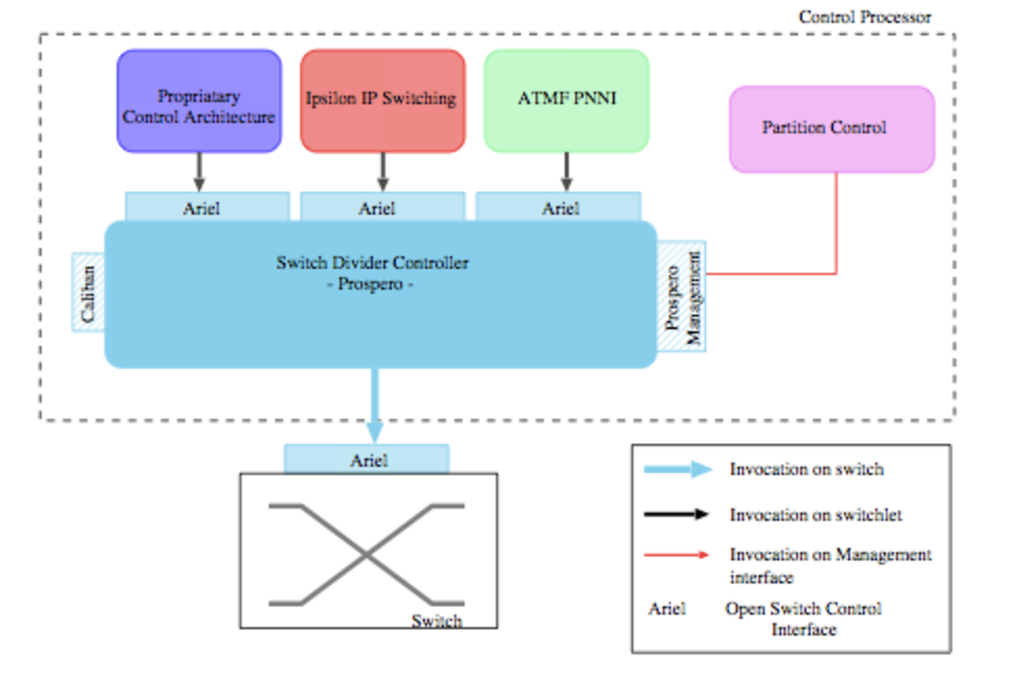
\includegraphics[width=0.7\textwidth]{Background/BackgroundFigs/tempest_arch}
\caption{Tempest switch architecture~\cite{UCAM-CL-TR-450}}
\label{fig:background:tempest_arch}
\end{center}
\end{figure}

\todo{add GSMP protocol reference}
An effort to network programmability in ATM network was also developed by the
University of Cambridge, as part of the DCAN project~\cite{dcan}.  The main
focus of the DCAN project was the development of a dynamic network control plane
which could virtualise an ATM network.  In~\cite{Rooney1998}, the authors
present Tempest, a novel ATM switch architecture, which achieved the goals of
the DCAN project.  Tempest provides a clear separation between the control and
forwarding plane of a network device.  The control plane of network devices, is
centralised in a single programmable entity, which implements intelligent and
dynamic forwarding.  The implementation of Tempest is logically divided between
three abstractions, depicted in Figure~\ref{fig:background:tempest_arch}. The
Figure presents how a single switch is able to function in parallel as an IP
router, an ATM switch and a Hollowman controlller~\cite{Rooney1997}, a devolved
ATM control framework. 

\paragraph{Prospero Switch Divider} 

The \emph{Prospero} abstraction provides a mechanism to virtualise ATM switch
resources. Prospero provides a resource control interface, which can divide
switch resource between multiple virtual switches, called \emph{switchlets}.  A
switchlet controls a subset of the switch ports, VCI and VPI mappings, packet
buffer and bandwidth. For packet buffer and bandwidth virtualization, Prospero
uses the ATM defined QoS  principles. In addition, Prospero is responsible to
map the control interface, exposed to controllers, with the underlying switch
functionality. 

\paragraph{Ariel Switch Independent Control Interface} 

Switchlets expose forwarding control through the Ariel Interface. Ariel
Interface organises network control through five control objects:
\emph{Configuration}, \emph{Port}, \emph{Context}, {\it Connections}
\emph{Statistics} and \emph{Alarms}.  Configuration provides details for the
switch configuration, Port provides primitive controllability of ports
(e.g.~state, loopback functionality), Context enables QoS policy control,
Connections expose control of VPI/VCI mappings, Statistics exposes packet and
byte counters and Alarms push state change notifications to the controller. Any
Tempest switch runs an Ariel server and translates Ariel request to Prospero
control requests. 

\paragraph{Caliban Switch Management Interface}

Apart from control capability support, Tempest also supported evolved network
management, through the Caliban interface. The interface functionality is
similar to the SNMP protocol. Caliban provides fine level SNMP-style
information, but can also provide higher level aggregation operations over the
switch state. 

In addition to the redefinition of the network control abstraction, Tempest also
proposed a relaxed network resource management scheme.  Specifically, the
architecture proposed a measurement-based admission control mechanism for
circuit establishment~\cite{Lewis1998}. The measurement scheme redefined the
static resource allocation scheme in ATM network, and used effective bandwidth
measurement techniques to estimate available resources.  This admission control
scheme provided higher utilisation of network resources, while providing QoS
guaranteed. 

Tempest defined a highly efficient network control abstraction. The
effectiveness of the control abstraction motivates modern network control
approaches, like SDN, to reimplement it over Ethernet devices.  In addition, the
simplicity of the control abstraction, permitted integration of the technology
with existing forwarding devices  and enabled line rate forwarding and efficient
resource control.  Nonetheless, its strong reliance on the ATM technology made
the approach less relevant for the modern Ethernet-dominated networks~\cite{Crosby2002}. 

\subsection{SDN}\label{sec:background:sdn} 

A recent attempt to develop a framework for distributed and scalable control is
the Software Defined Networking (SDN) paradigm. SDN~\cite{sdn} enables the clean
separation between the control and the forwarding plane of a network device. The
control plane logic is implemented in a separate programmable device and a well
defined protocol establishes the inter-connection between the two devices. 

The SDN approach is inspired by relevant earlier attempts in network
programmability(Active Networks and DCAN), but follows an evolutionary approach.
SDN supports existing network data protocols and focuses to provide the
mechanism to development custom forwarding mechanisms.  The paradigm is
motivated by two observations in current network technologies.  Firstly, the
evolution of computer networks has reduced the applicability of the multi-layer
network abstraction. Production networks contain middleboxes (e.g.~firewall,
NAT, layer-5 switches) that operate on multiple layers of the network and engage
extensively in layer violation.  Such devices cannot integrate with existing
control mechanisms, while they remain transparent by the end-hosts. The SDN
paradigm aims to provide a new unifying cross-layer control model that can
integrate control for such devices.  Secondly, although network complexity has
increased, network devices still use stand-alone configuration mechanisms (e.g.
remote logic, CLI interfaces) and global network policies must be decomposed by
network administrators in individual network device policies, to fit the
existing control abstraction. In order to modify network-wide configuration,
network administrators must login over telnet or use a web interface to
configure each device manually.  In addition, network vendors develop
proprietary control protocols which reduce device interoperable.  SDN enables
management centralisation, while the flexibility of the control abstraction
enables control innovation mechanisms that match network environment
requirements.

The SDN paradigm was highly successful in the network community and within a few
years since its introduction, network vendors engaged in the development of
production-level implementations. In addition, the research community has
developed a number of interesting SDN architectures which address several network
problems. The \of protocol is currently the pre-dominant implementation of the SDN 
paradigm.

\subsubsection*{\of protocol} 

\begin{figure}
  \begin{center}
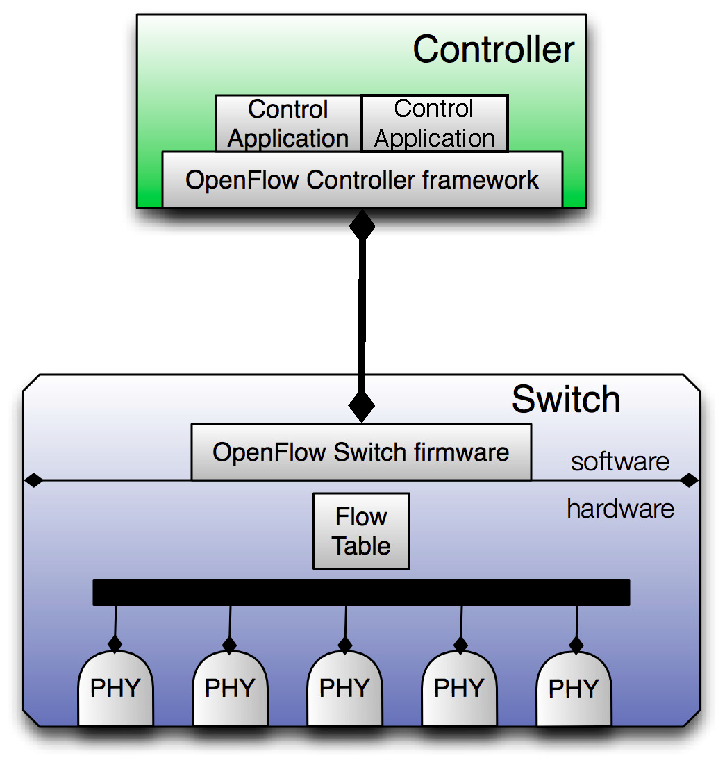
\includegraphics[width=0.5\textwidth]{Background/BackgroundFigs/openflow-schema}
\caption{A schematic representation of a basic \of setup}
\label{fig:background:openflow-schema}
\end{center}
\end{figure}
\begin{table}
  \begin{minipage} []{0.49\textwidth} 
    \begin{tabular}{|p{4cm}  | p{2cm} |} 
      \hline
      Field & OpenFlow Version \\ 
      \hline
      src \& dst MAC addr. & 1.0~\footnote{SInce version 1.1 the protocol
        permits masked mac address matching} \\ \hline
      input port & 1.0 \\ \hline
      VLAN ID & 1.0 \\ \hline 
      VLAN PCP & 1.0 \\ \hline
      MPLS label & 1.1 \\ \hline
      MPLS class & 1.1 \\ \hline 
      IPv4 src/dst addr. & 1.0 \\ \hline
      IPv4 proto & 1.0 \\ \hline
      ARP opcode & 1.0 \\ \hline 
      ARP src/dst IPv4 address & 1.0 \\ \hline 
      ARP src/dst MAC address & 1.2 \\ \hline 
    \end{tabular}
  \end{minipage}
  \begin{minipage} []{0.49\textwidth} 
    \begin{tabular}{|p{4cm}  | p{2cm} |} 
      \hline
      Field & OpenFlow Version \\  \hline
      IPv4 ToS & 1.0 \\ \hline 
      ICMPv4 Type \& Code & 1.0 \\ \hline
      TCP/UDP/SCTP src/dst port & 1.0 \\ \hline
      metadata & 1.1 \\ \hline
      IPv6 src/dst addr. & 1.2 \\ \hline
      IPv6 flow label & 1.2 \\ \hline
      ICMPv6 type \& code & 1.2 \\ \hline
      ICMPv6 Network Discovery target address & 1.2 \\ \hline
      ICMPv6 Network Discovery src/dst MAC address & 1.2 \\ \hline
    \end{tabular}
  \end{minipage}
    \caption{\of tuple fields} \label{tbl:background:openflow_tupple}
\end{table}
  \begin{table}
  \begin{minipage} [b]{0.49\textwidth} 
    \begin{tabular}{| p{4cm} | p{6cm}  | p{1.5cm} |} 
      \hline
      Field & operation & OpenFlow Version \\ \hline
      OUTPUT & output packet to a port & 1.0 \\ \hline
      SET\_QUEUE & output packet to a port queue & 1.0 \\ \hline
      SET\_VLAN\_VID & modify VLAN id & 1.0 \\ \hline 
      SET\_VLAN\_PCP & modify VLAN PCP & 1.0 \\ \hline
      SET\_DL\_SRC SET\_DL\_DST & modify src/dst mac addr. & 1.0 \\ \hline
      SET\_NW\_(SRC,DST) & modify IPv4 src/dst addr. & 1.0 \\ \hline
      SET\_NW\_TOS & modify IPv4 ToS & 1.0 \\ \hline
      SET\_NW\_ECN & modify IPv4 ECN bits & 1.1 \\ \hline
      SET\_TP\_(SRC,DST) & modify TCP/UDP/SCTP src/dst port & 1.0 \\ \hline
      COPY\_TTL\_(OUT,IN) & copy TTL value for IPv4 tunnels & 1.1  \\ \hline
      SET\_MPLS\_LABEL & modify MPLS label & 1.1 \\ \hline
      SET\_MPLS\_TC & modify MPLS traffic class & 1.1 \\ \hline
      (SET,DEC)\_MPLS\_TTL & modify/decrement MPLS TTL & 1.1 \\ \hline
      (PUSH,POP)\_VLAN & Add/remove a VLAN header & 1.1~\footnote{\of 1.0 defined
        a primitive to remove a VLAN header only} \\ \hline
      (PUSH,POP)\_MPLS & add/remove MPLS tag & 1.1 \\ \hline
      (SET,DEC)\_NW\_TTL & modify/decrement IPv4 TTL value & 1.1 \\ \hline
      (PUSH,POP)\_PBB & remove/add a PBB service tag & 1.3 \\ \hline

    \end{tabular}
  \end{minipage}
  \caption{\of available packet actions} \label{tbl:background:openflow_actions}
\end{table}




\of is an instantiation of the SDN paradigm. The protocol was originally
developed by the \of Consortium, a collaborative organisation of academic
institutes, but soon its development was adopted by the ONF, a standards
definition committee comprised of academic institutions and network vendors. \of has
been a highly successful approach to network control. A number of vendors
has introduced support of the protocol in their products
while there are already \of deployments in enterprise networks~\cite{google_of,Kobayashi:vn}.

A representation of a simple \of topology is presented in
Figure~\ref{fig:background:openflow-schema}. A minimum \of topology consists of
two entities: the \emph{Controller} and the \emph{Switch}. The Controller
implements and disseminates the control logic of the network to the switches
over a control channel. A controller can control multiple switches. In addition, 
the network community has developed a number of programming environments to
develop \of control applications. Such programming environments provide a 
higher level abstraction over the \of protocol and reduce the exposure of
the developer to the run-time details~\cite{nox,floodlight,nodeflow}.

The switch entity is responsible to transform \of protocol operations in data
path policy modifications. The \of functionality is split between the data and
control layer of the switch. In the data layer, the protocol implements a simple
packet processing algorithm.  For each packet, the hardware extracts a number of
fields and matches them against the entries of a \emph{Flow Table}.  The Flow
Table is a memory abstraction which contains forwarding policy. It comprises of
flow entries which conceptually consist of three parts: the flow tuple, the flow
statistics and the flow action list.  The flow tuple synthesizes a flow
description using all the significant packet header fields.  We present the list
of fields in Table~\ref{tbl:background:openflow_tupple}.  The protocol
associates with each flow tuple a flow mask, which permits field wildcarding in
a flow definition.  Flow statistics store flow packet and byte counters. The
action list, contains the list of actions that should be applied on every
matched packet.  We present in Table~\ref{tbl:background:openflow_actions} the
packet processing actions defined by the \of protocol.  On a packet reception,
if a matching flow is found in the flow table, then the flow statistics are
updated and the action list is applied on the packet. If there aren't any
matching flow entries, the packet propagates as an exception to the control
layer of the switch.  The control plane of the switch implements the translation
of the \of protocol into data path modifications.  It provides access and
modification functionality to the switch configuration and the flow table. The
switch is able also to propagate autonomously information and exceptions 
to the controller. 

The ensemble of a flow table and a set of switch ports comprises an \of
\emph{datapath} and is the core abstraction for network control.  The protocol
defines a number of protocol message types to manage datapath resources. \of 
control operations can be grouped in two categories:
\emph{Forwarding control} and \emph{Switch configuration}. In the rest of the
section we present how this functionality is addressed by \of messages and how
this mechanism is evolved over the different versions of the protocol. We
focus our protocol presentation over the 1.0 version of the protocol.
ONF has releases three revisions of the
protocol, version 1.1, 1.2 and 1.3, which change significantly the protocol
specification. Nonetheless, the majority of production systems are predominantly 
version 1.0 compliant.
% the \of protocol version 1.0 to control a
% network. This version was introduced in 2009 and is currently the market default
% support. Since then, the ONF steering board has released three more version,
% 1.1, 1.2 and 1.3, which redefine to a great extend the default processing logic
% of the abstraction. Following, we will present the core mechanisms of version
% 1.0 and describe in a higher level the incremental differentiations introduced
% in the following versions of the protocol. 

\paragraph{Forwarding control}

\of provides fundamentally two modes of control: \emph{reactive} and 
\emph{proactive} control. In the reactive approach, the switch is configured to
forward every unmatched packet to the controller, and the controller is
responsible to respond with appropriate modification in the flow table. The
protocol defines the {\tt pkt\_in} message type, that can propagate the header
of a packet to the controller, and the {\tt flow\_mod} message type, that can
manipulate flow table entries. The reactive control approach provides 
fine control over the traffic dynamics, but, depending on the deployment
environment, can introduce significant load on the control plane. In the proactive
approach, the controller is responsible to pre-install all required flows in the
flow table and avoid any packet handling exceptions. Because this approach
lucks data plane feedback, the \of protocol provides the {\tt stats\_req/stats\_resp}
and {\tt aggr\_stats\_req/aggr\_stats\_resp} message types. These message types allow
the controller to poll dynamically for flow statistics and infer network
resource allocation. In order to ensure atomicity in the protocol, the protocol
also define a {\tt barrier\_req/barrier\_reply} message type, which provides a synch 
point between the controller and the switch. A {\tt barrier\_reply} is send by a
switch as a response to a {\tt barrier\_req} from the controller, only if all previous 
operations are processed. 
Finally, the \of protocol provides two additional message
types to increase users ability to interact with the forwarding plane: the {\tt
  pkt\_out} and the {\tt flow\_removed}. The {\tt pkt\_out} message enables the
controller to inject traffic in the data plane and the {\tt flow\_removed} message
can notify the controller when a flow entry is removed from the flow table. The
protocol defines flow timers and the switch can remove a flow with an expired
timer. 

\paragraph{Switch configuration} 

Apart from the control of the flow table, the \of protocol provides switch
configuration capabilities. A controller can use the {\tt
  switch\_config\_req/switch\_config\_resp} message types, to discover switch \of
operation support.  In addition, the protocol provides capabilities to control
port state with the {\tt port\_mod} message type. The switch is also able to
notify the controller when a port changes its state (e.g.~link is detected to be
inactive in the physical layer) with the {\tt port\_status} message. In the
recent revisions of the protocol, the steering committee has introduced the
capability to control per port traffic shaping queues. 

\paragraph{Protocol evolution} 

Since the specification of the version 1.0 of the protocol, the \of steering
committee has produced 3 non-backward compatible revisions of the protocol. The
updates in the protocol are motivated both by the osmosis between the hardware
and software \of community, as well as, by the introduction of new deployment
use cases. 

Version 1.1 of the protocol introduces a number of modification in the main
protocol pipelne in order to improve the integration of the protocol with the
silicon functionality. Firstly, the default packet processing algorithm is
differentiated. A switch can accommodate multiple flow tables and the lookup
process searches sequentially each of the tables for flow matches. The packet
must have a match in each of the tables otherwise a {\tt pkt\_in} message is
generated. In addition, in order to persist partial results between tables, the
protocol define a 64-bit metadata field and the action list is augmented with
operations over the metadata field, as well as, over the table search process
(e.g.~terminate lookup, skip table).  Secondly, the protocol introduces a
primitive to express multipath support in the protocol. This functionality is
exposed through a group table abstraction.  Group table entries contain a set of
buckets containing flow actions and an assigned output port. A controller in the
action of a flow can forward packet to a group entry. The goup selection action
can select to forward the packet either to all the buckets of the entry (ALL) or
select randomly a bucket, in a manner similar to the Equal Cost Multiple Path
routing (ECMP)~\cite{RFC2992} functionality, (SELECT) or select a specific
bucket (INDIRECT) or forward packet to the first group entry for which the
output port can forward packet (FAST\_FAILOVER).  Thirdly, the protocol
introduces MPLS matching support and manipulation.

Version 1.2 of the protocol extends data plane protocol support. This revision
introduces support for IPv6 and Provider Bridge Network (PBB - Mac-in-Mac)
traffic. In addition the protocol defines a new TLV format for flow Match
definition, in order to relax the \of tuple definition.  Finally, the protocol
defines a model to enable multi-controller connectivity for switches.
Multi-Controller schemes provides resilience to the control of the network. 

In Version 1.3 the protocol definition introduces protocol support of QoS
control. The protocol defines a new table abstraction, the metering table, which
contains queue definitions. In addition, this protocol definition introduces the
idea of multiple parallel control channels towards the same controller, in order
to parallelize {\tt pkt\_in} transmission, and defines a mechanism to support
message fragmentation.  

Because the recent versions of the protocol has become complex, the vision of
future \of deployment, is to differentiate switch abstraction and develop
diverse product ranges that will provide optimized support for a subset of the
protocol. 


\section{SDN applications} \label{sec:background:ofapp}

\begin{table}
  \center
  \begin{tabular}{|c  | l |}
    \hline
    Language & controller \\
    \hline
    Python & NOX~\cite{nox}, POX~\cite{pox}, Pyretic~\cite{Monsanto13} \\
    C++ & NOX~\cite{nox} \\
    JAVA & Maestro~\cite{cai2011}, Floodlight~\cite{floodlight} \\
    Haskell & Nettle~\cite{nettle} \\
    C & Mul~\cite{mul} \\
    Javascript & Nodeflow~\cite{nodeflow} \\
    Ruby & Trema~\cite{trema} \\
    \hline

  \end{tabular}
  \caption{List of \of controller organised by programming language}
  \label{tbl:openflow-controller}
\end{table}
 
\begin{table}
  \center
  \begin{tabular}{|c  | c | c |}
    \hline
    Vendor & Model & \of version \\
    \hline

    HP & 8200zl, 6600, 6200zl, 5400zl, and 3500/3500yl & v1.0 \\
    Brocade & NetIron CES 2000 Series & v1.0 \\
    IBM & RackSwitch G8264 & v1.0 \\
    NEC & PF5240, PF5820 & v1.0 \\
    Pronto & 3290, 3780 & v1.0 \\
    Juniper & Junos MX-Series & v1.0 \\
    Pica8 &  P-3290, P-3295, P-3780 and P-3920 & v1.2 \\
    \hline
  \end{tabular}
  \caption{List of hardware switches with \of support }
  \label{tbl:openflow-switch}
\end{table}
 
The introduction of the SDN paradigm proved to be extremely successful not only
in the research community, but also in the network industry. Already a number of
vendors provide production-level hardware support for
SDN~(Table~\ref{tbl:openflow-switch}, and the SDN community provides \of support
for most programming languages~\ref{tbl:openflow-controller}.  In order to
exhibit the class of problems which can be tackled by appropriate design of the
control plane, in this section we present applications of the SDN paradigm in
different network problems. 

\subsection{Network Virtualisation}

The introduction of OS virtualization and the subsequent rise of the cloud
computing paradigm has created new opportunities for computer science to reduce
infrastructure costs and create new highly resilient system architectures.
Although platforms like Xen provide strong guarantees on resource allocation and
performance isolation on the OS level, there is still a significant gap in
network virtualisation.  The introduction of the SDN paradigm provides novel
capabilities to the research community to develop new network abstractions and
expose direct network control to tenants, while assuring the correct
functionality of the network. 

The first attempt to enable network virtualisation
in the data center was through the FlowVisor project~\cite{flowvisor-ccr}.
FlowVisor function as a \of proxy and sits between the \of switches and the \of
controller. By appropriate message processing, a network topology discovery
mechanism and a resource management policy, FlowVisor aggregate control over a
set of switches and exposes a single virtual switch 
abstraction. The administrator can partition the \of tuple and delegate
network control to different controllers, thus allowing data center tenants to
control traffic for their own subnet and VM group. FlowVisor is currently
adopted by BigSwitch and developed as a product. In~\cite{Corin12} the authors
develop an extension for the FlowVisor  platform, which enables
topology virtualisation capabilities. In~\cite{Drutskoy13} the authors present FLowN,
a network virtualisation mechanism which provides full control of \of tupple to
all tenants and multiplexes user traffic using VLAN tags. FlowN, in addition,
removes the latency incurred by control proxy by encapsulating the control
transformation process in the programming library. Furthermore,
state synchronisation is implemented through an SQL database, which
is used by the programming library to transform \of messages. Finally, Nicira has
develop Nicira Network Virtualization Platform (NVP), which claims to provide
full network virtualisation and control isolation. Nonethless, the product is
proprietary and implementation details remain undisclosed.  

\subsection{Security and Access Control}

As we have discussed in the introduction of this thesis, network security has
become a significant requirement for modern network operability. In order to
improve network security, we require novel control plane architectures which are
inherently secure. SDN provides a mechanism to enable fast prototyping of secure
network architectures, while the high programmability of the controller allows
traffic-inspecting security application integration with the control logic of
the network.  In an early attempt to define the SDN abstraction, researchers in
Stanford developed the Ethane system~\cite{casado07:_Ethan}. Ethane defines a
simple policy expression language which uses as first-class object user
identities and network services, and defines the interconnection ability between
the two. SDN provides also the means to develop lossless, highly performant and
programmable network trace collection mechanisms. In~\cite{Ballard10}, the
authors present OpenSAFE, a policy expression language which allows a network
manager to define policies to intercept and inspect network traffic, enabling a
highly flexible and dynamic network monitoring applications. Finally,
in~\cite{Porras12}, the authors present FortNOX, a mechanism which enables
secure interaction between the control applications of a network. FortNOX
enables users to assign priorities and roles to controlling applications and
implements a simple resolution mechanism when two applications introduce
contradicting network policies. 
 
\subsection{Load Balancing}

The introduction of network services with global audience has created a
requirement for IP indirection mechanisms, to distribute network load between
servers in server farms and cloud computing infrastructures. A common approach
to address this problem is through proprietary load balancing devices that
function on the gateway of the server farm and distribute dynamically user
request between servers. The introduction of the SDN abstraction integrates this
indirection functionality in the network fabric.  In~\cite{Wang11}, the authors
present a framework for in-network load balancing functionality. The system
preinstall wildcard rules to forward new flows to a specific server. As the
server load changes, the control dynamically modifies the wildcard coverage and
redirects new flows to less utilised servers.  In~\cite{Handigol09,Handigol10},
the author present a reactive approach to the problem. In the Plug-and-Serve
architecture, the controller is responsible to handle each new connection and
forward traffic to a specific server, based on the allocation algorithm and the
current load of the system.

\subsection{Inter-domain and Intra-domain Routing}

In the context of network control, the SDN paradigm has also been proposed in
order to improve the performance of existing control plane protocols.
In~\cite{Rothenberg12}, the authors present an integration of the
Quagga~\cite{quagga} routing framework with the \of protocol, in an effort to
revisit the Route Reflector idea in BGP routing~\cite{RFC4456}. Furthermore, In
an effort to reduce the impact of routing instabilities of the BGP protocol, the
authors in~\cite{Kotronis12} propose a mechanism to offload BGP routing to third
party entities and use the \of abstraction to propagate resulting FIBs to the 
outsourced-network devices.

The programmable nature of the SDN paradigm and its ability to centralise
network control has also motivated explorations on network state compression.
In~\cite{Sarrar12}, the authors present a library which exposes a FIB
abstraction over the \of abstraction to routing applications.  The library at
run-time analyses the resulting FIB, as well as, the traffic pattern and
calculates an minimum set of flow entries which can server a specific subset of
the traffici on the fast-path of the network.  In a similar effort, authors
in~\cite{Yu10} present DIFANE, a routing mechanism which uses valiant
inter-routing, in an effort to compress the average FIB table size within the
network. The proposed mechanism uses the \of abstraction in order to partition
effectively the network and disseminate forwarding state across the network
devices. 

\subsection{Network Management}

One of the core goals of the SDN paradigm is to provide the development
environment for innovative management mechanisms which ease the network control
task. One of the first application of the SDN paradigm was introduced
by~\cite{Koponen10} within the context of the Onix control platform. Onix
provides a centralised control abstraction to network developers, over which
they can program their network control logic. The abstraction encapsulates a
control state distribution mechanism which enables seamless distributed
execution of code. 

In a similar effort a number of novel programming languages has be proposed to
formalise the control plane requirements.  In~\cite{Foster11} the authors
present the Frenetic programming language, a declarative language to define
network control policy. The language encapsulates in the programming model
significant network control programming requirements, like race conditions
abstraction mechanisms. Furthermore, in~\cite{Monsanto12a} the authors describe
NetCore, a novel policy expression language which enables users to express their
control logic. At run-time the policy adapts to the network traffic and topology
in an effort to optimizes the installed state within the network.  The NetCore
abstraction is further enhanced with the ability to provide verifiable control
policies in the network, as presented in~\cite{Guha13}. In addition,
in~\cite{Monsanto13} the authors define a framework build on top of the NetCore
language which enables seamless integration of the control logic between
different control applications and reduces the complexity to integrate
individual control applications in the network. Such control abstraction have
also been discuss in the context of network control logic updates.
In~\cite{Reitblatt12}, the authors present a verifiable mechanism to upgrade the
network control logic without any network disruption. Finally,
in~\cite{Voellmy12}, the authors present a novel declarative policy language
which builds on top of the reactive functional programming model and provides a
highly flexible architecture to develop novel control management systems. 

\subsection{Energy}

In the recent years energy consumption has become an important measure of
efficiency for a system architecture. Currently the network is estimated to
contribute approximately 20\% of the total power consumption of a data-center.
Unlike CPUs which can reduce power consumption when idle, network cards exhibit
a constant high power consumption, due to the constant requirement for medium
sensing and physical layer frame synchronisation. As a result the most efficient
mechanism to reduce network power consumption is to shutdown interfaces.
In~\cite{Heller10}, the authors present a power-aware control plane
architecture, build on top of the \of abstraction. The application takes
advantage of link redundancy and turns off interfaces when network utilisation
is low. 

\subsection{Network Debugging and Measurement}

The SDN paradigm, as well as, the \of abstraction provide novel mechanisms to
troubleshoot a network. In~\cite{Wundsam11}, the authors present a mechanism to
intercept and record traffic flows from a network. Recorded flows can be
replayed within the network, in order to detect policy misconfigurations which
create functionality problems. In a similar effort, in~\cite{Handigol12} the
authors present ndb, a control plane debugger which enables users to register
data plane breakpoint conditions and receive rich control plane run-time
informationi when this conditions are met. Finally, a number of applications
have been proposed to enable control plane monitoring in order to detect
potential networks misconfigurations. In~\cite{Khurshid12}, the author present
an \of proxy service which detect flow modifications which create
forwarding policy inconsistencies.  In~\cite{Canini12}, the authors present a model
checking mechanism which uses symbolic execution to detect flow modifications
which create significant inconsistencies in the data plane forwarding.
Debugging applications of the \of abstraction have been also proposed in the
context of home networks.  In~\cite{Calvert10}, the authors proposed a network
controller which enables precise network logging by the home router, in
order to aid ISPs to troubleshoot connectivity problems. 

% \cite{opentm-pam}, 
%   OFRewind, ndb, end, VeriFlow~\cite{Khurshid12}
% Home instrumenting~\cite{Calvert10}, An \of-based instrumentation
%         router for home networks. ISP can receive accurate network information 
%         from the home network and troubleshoot easier home problems.

\subsection{Resource Control}

The high reactivity of the SDN paradigm 
enables fine level resource control integrated with the control plane.
Already a number of control designs applicable in the datacenter environment
have been proposed by the research community. 
In~\cite{Al-Fares10} the authors present Hedera, a
novel control architecture for datacenters which improves the network
utilisation in comparison to the popoular ECMP~\cite{RFC2992} network load
balancing mechanism. The system uses the flow statistics mechanism provided by
the \of abstraction and at run time discovers progressively network-limited
flows which are rerouted over underutilised network paths. In a similar
effort, the authors in~\cite{Benson11} present a network load distribution mechanism
with a higher granularity on short-lived flows. Furthermore,
in~\cite{Even12} the authors propose a network embedding mechanism which is able
to define job assignments in a datacenter and provide strong guarantees on
network resources.

Resource control has also been proposed in the context of home network.
In~\cite{Yiakoumis11} the authors propose the deployment of network
virtualisation in the home network to improve resource allocation on the edges,
as well as,  enable core infrastructure sharing between ISPs.
In~\cite{Yiakoumis12} the authors evolve this idea and introduce a simple user
interface which can translate user resource requirement into ISP wide network
policies. 

\subsection{Mobility}

The SDN paradigm has found excellent applicability in addressing the increased
control plane requirement in mobile networks. In~\cite{Huang10} the authors
present PhoneNet, an application development framework which provides the
ability to applications to setup multicast groups in the network through the
controller. In~\cite{Yap09,Yap10} the authors present OpenRoads, a network
control plane for wireless network which enables seamless Access Point~(AP)
hand-overs for devices, as well as, network virtualisation.  Finally, the
authors in~\cite{Li12} discuss SDN abstraction requirements for cellular
networks.

\subsection{Network Simulation}

The capability of the SDN paradigm for fast network functionality prototyping
provides a novel experimentation mechanism for network researchers.  Currently a
number of large-scale shared infrastructures are built and maintained by
research organisation. The GENI testbed~\cite{geni} in the US funded by the NSF
and the Ofelia testbed~\cite{ofelia} in the EU funded by the FP7 framework
provide network and computing resource to run large-scale experiments
for free. Furthermore, a number of \of-based frameworks has been developed
for scalable network experimentation.
In~\cite{Erickson11} the authors present Virtue, a large-scale emulation
framework which uses the Xen virtualization platform and the \of protocol to
enable user experimentation with network topologies and VM placements in a
multi-tenant data center environment.  In addition, the Mininet
platform~\cite{Lantz10,Handigol12} has been developed by researchers in Stanford
to enable scalable experimentation with the \of protocol. Mininet uses the
LXC~\cite{lxc} linux user-space virtualisation framework to run multiple virtual
machine in a single host and experiment with network functionality. Mininet has
been used in the Computer Science department in Stanford to aid the introduction
of students with recent research efforts in computer networks~\cite{cs244}. 

\section{Conclusions}

In this Section we have provided an in-depth analysis of network control
mechanisms.  We motivate our discussion in network control by presenting a
generic architectural model for network devices and focus on the inherent
limitations for network control. Furthermore, we present the current control
plane mechanisms in production networks and, motivated by the limitations of
these mechanisms, we present three control mechanisms, proposed by the research
community, which aim to improve the respective limitations. Finally, we provide
an extensive presentation of recent efforts to improve modern network
functionality through control plane redesign. In the next chapter we present an
extensive study on the scalability of the SDN paradigm. 
